\documentclass{ntuthesis}

\usepackage{times}
\usepackage{verbatim}
\usepackage{color}
\usepackage{url}
\usepackage{graphicx}
\usepackage{array}
\usepackage{wallpaper}
\usepackage{hyperref}
\usepackage[printwatermark]{xwatermark}
\usepackage{graphicx}
\usepackage{tikz}

% Using the tex-text mapping for ligatures etc.
\defaultfontfeatures{Mapping=tex-text}

% Set the default fonts
\setmainfont{Times New Roman}
\setCJKmainfont[AutoFakeBold=true,AutoFakeSlant=true]{標楷體}
%\setCJKmainfont[BoldFont={粗楷體},ItalicFont={斜楷體}]{標楷體}

\ifdefined\firstpage

  \ifdefined\withwatermark
    \newsavebox\mybox
    \savebox\mybox{\tikz[opacity=0.5]\node{\includegraphics{watermark.pdf}};}
    \newwatermark*[allpages,xpos=6.1725cm,ypos=10.5225cm,scale=0.5]{\usebox\mybox}
  \fi

  % digital object identifier
  \ifdefined\withdoi
    \insertdoi
  \fi
\fi

\makeatletter
\AtBeginDocument{
  \hypersetup{
    pdftitle={\@titleen},
    pdfauthor={\@authoren},
    pdfsubject={\@typeen{} \@classen},
    pdfkeywords={\@keywordsen}
  }
}
\makeatother

% Your information goes here
% author: Tz-Huan Huang [http://www.csie.ntu.edu.tw/~tzhuan]

% ----------------------------------------------------------------------------
% "THE CHOCOLATE-WARE LICENSE":
% Tz-Huan Huang wrote this file. As long as you retain this notice you
% can do whatever you want with this stuff. If we meet some day, and you think
% this stuff is worth it, you can buy me a chocolate in return Tz-Huan Huang
% ----------------------------------------------------------------------------

% Syntax: \var{English}{Chinese}
\university{National Taiwan University}{國立臺灣大學}
\college{College of Electrical Engineering and Computer Science}{電機資訊學院}
\institute{Department of Computer Science and Information Engineering}{資訊工程學系}
\title{In-Car Face Detection under Various Lighting Situations}{在不同光照下進行車內人臉辨識}
\author{Yi-Chen Chuang}{莊宜蓁}
\studentid{R07922066}
\advisor{Yung-Yu Chuang, Ph.D.}{莊永裕 博士}
\defenseyear{202?}{1??}
\defensemonth{????}{?}
\defenseday{??}
\doi{doi:10.6342/NTU202?XXXXX}
\keywords{Face Detection, In-Car Face Detection, Image Enhancement, Normalization}{人臉偵測, 車內人臉偵測, 影像增強, 正規化}


\begin{document}

\frontmatter

\makecover

\ifdefined\excludefirstpage

  \ifdefined\withwatermark
    \newsavebox\mybox
    \savebox\mybox{\tikz[opacity=0.5]\node{\includegraphics{watermark.pdf}};}
    \newwatermark*[allpages,xpos=6.1725cm,ypos=10.5225cm,scale=0.5]{\usebox\mybox}
  \fi

  % digital object identifier
  \ifdefined\withdoi
    \insertdoi
  \fi
\fi

\makecertification

\input{acknowledgements}
\begin{abstractzh}
近年來隨著智慧型汽車相關技術的成熟,車內人臉辨識逐漸受到重視。然而一般的人臉偵測模型尚無法在車內人臉辨識上獲得較好的結果。其原因我們推測為車內人臉辨識會碰到較多在不同光照下的例子,而一般的人臉偵測模型著重於大多數情境下的表現結果,經常忽略在較極端光照下的例子所致。在本論文中我們試著消除不同光照對圖片造成的影響。我們提出一個訓練架構來訓練出能夠對輸入資料在偵測前進行正規化處理的正規器,並將此正規器和人臉偵測器接在一起進行端對端訓練優化。我們的方法在基線做得最差的測試情境中相比基線結果進步了 47.27\%。

\bigbreak
\noindent \textbf{關鍵字:}{\, \makeatletter \@keywordszh \makeatother}
\end{abstractzh}

\begin{abstracten}
As intelligent vehicle technologies become mature, in-car face detection gradually draws everyone's attention. However, general face detection models have yet to perform good when it comes to in-car face detection. We guess the reason is that while in-car face detection has to deal with more cases from various lighting situations, general face detection tends to focus on performing good on major cases and often ignores cases under extreme lighting situations. In this thesis, we tried to remove the effect lighting had on images. We proposed a training architecture to train a normalizer to normalize input images before getting detected, jointed it with a face detector and did end-to-end training for optimization. Our method outperformed baseline by 47.27\% in the test scenario that baseline performed worst on.

\bigbreak
\noindent \textbf{Keywords:}{\, \makeatletter \@keywordsen \makeatother}
\end{abstracten}


\tableofcontents
\listoffigures
\listoftables

\mainmatter

% Your thesis goes here
\chapter{緒論}
\label{c:intro}

人臉偵測一直以來都是深度學習和電腦視覺領域中一個重要的議題。經過了幾年的研究,人臉偵測也漸趨成熟,得以被應用在更多領域中。而其中一個新興的領域便是智慧型汽車。汽車駕駛和我們的生活息息相關,一直以來各大車廠以及研究人員都在不斷研究如何讓駕駛汽車變得更加方便和安全,因而研發出各項技術,如智慧駕駛輔助、自動駕駛等等。隨著這些技術的成熟,車內影像的應用也逐漸受到關注,而對車內人臉的偵測便是一項重要的核心技術。在車內進行人臉偵測能夠協助定位出駕駛與乘客的臉部位置,並能夠接著進行後續的其他應用,如進行身分辨識、偵測駕駛臉部朝向等等,能夠使駕駛汽車更加安全。

然而在現階段,人臉偵測的研究尚無法直接應用於智慧型汽車這個領域。在測試下我們發現,一般的人臉偵測模型做在車內人臉上的表現不如我們預期。車內人臉偵測的結果對後續的相關應用十分重要,因此我們認為如何改善偵測的結果是相當值得研究的。在經過觀察之後我們發現,車內人臉偵測和一般人臉偵測相比有更多在多樣光照下的例子。一般人臉偵測的研究大多著重於提升大多數情境下的表現結果,經常忽略在較極端光照下的例子,因此其在車內人臉的偵測上便表現得較不如預期。

在本研究中,我們在進行人臉偵測前用正規器先對輸入圖片進行正規化處理 (Normalization),並提出了針對此正規器的訓練架構。我們希望能透過消除光照對輸入圖片所造成的差異,來改善模型在人臉偵測上的表現結果。

在接下來的章節中我們會陸續提到以下內容:
在第~\ref{c:related}章,我們會介紹和本研究相關的其他研究,包含了人臉偵測、低光照下的人臉偵測和影像增強。在第~\ref{c:method}章,我們會先闡述我們確定本研究中目標的過程,然後詳細說明在本研究中所使用的方法細節。在第~\ref{c:experiment}章,我們會說明我們在訓練和測試時使用的資料集和實驗設定,展示視覺和數據上的結果,並以實驗說明我們的方法中各個細節對實驗結果造成的影響。而在第~\ref{c:conclusion}章,我們會對本研究做出結論並提出未來努力的目標。

\chapter{相關研究}
\label{c:related}

\section{人臉偵測}
人臉偵測在電腦視覺領域是個發展成熟的議題,其因能被應用在諸多領域上而有很大的重要性。從以前到現在,人們使用各種不同的方式來解決這個議題。由 P. Viola~和M. J. Jones\cite{viola2004robust} 所提出的 Viola-Jones 目標檢測框架結合了積分圖 (Integral Image)、哈爾特徵 (Haar Feature)、自適應增強 (AdaBoost) 學習、將數個弱分類器級聯 (Cascade) 等概念,率先做到了實時性 (Real-Time) 高精度人臉偵測。而在卷積神經網路興起後,大家對人臉偵測的研究又更加熱烈。由 S. Zhang~\cite{zhang2017faceboxes} 所提出的 FaceBoxes 藉由在卷積層使用較大的步伐 (Stride) 快速將輸入縮小,在盡量不影響結果下減少輸出所需的頻道數,並搭配 Faster R-CNN~\cite{ren2015faster} 中核心的 RPN (Region Proposal Network) 網路和錨點 (Anchor) 的機制來做到高精度實時性的人臉偵測;由 J. Li~\cite{li2019dsfd} 所提出的 DSFD 強化圖片中被擷取的特徵並利用這兩組特徵來算出比單一一組特徵更準確的臉部位置;由 V. Bazarevsky~\cite{bazarevsky2019blazeface} 所提出的 BlazeFace 則使用了輕量化的網路和需要的運算處理較低的架構等,使人臉偵測能夠進一步被用於行動裝置的相關應用上。

\section{低光照下的人臉偵測}
人臉偵測並非只被應用於正常光照下的情境,有時候我們也會需要處理夜間等較有挑戰性的情境,而大家對於這樣的情境也各有不同的解決方案。S. W. Cho~\cite{cho2018face} 使用低光照下的圖片作為訓練資料,試圖使訓練時的情境接近測試時的情境以提升人臉偵測的準確率;M. K. Bhowmik~\cite{bhowmik2011thermal} 和 J. Kang~\cite{kang2015face} 分別使用了熱紅外光攝影機和近紅外光攝影機獲取非可見光照射下的資料,以避開低光照對圖片造成的影響;也有一些研究~\cite{cho2018face, li2017real, yang2020advancing}選擇對圖片進行增強,試圖還原在低光照下損失的色彩與細節以提升準確率。

\section{影像增強}
影像增強也是一個非常熱門的議題,人們透過增強圖片來還原圖片在低光照下損失的色彩與細節,讓圖片能被進行其他後續處理。較為傳統並廣為人知的作法有直方圖均衡化 (Histogram Equalization)~\cite{gonzales2002digital} 和珈瑪校正 (Gamma Correction)~\cite{gonzales2002digital}等,這些方法主要透過拉高像素間的對比來達到強調細節的效果。過去研究人員模仿人體視覺系統發展出視網膜增強算法~\cite{land1977retinex},近期也有研究受到這個算法的啟發。由 L. Shen~\cite{shen2017msr} 提出的 MSR-net 認為視網膜增強算法的架構和卷積神經網路相似,並將其演算法轉換成卷積神經網路;C. Wei~\cite{wei2018deep} 的研究將圖片分為光照 (Illumination) 和反射 (Reflectance) 兩部分,把光照部分增強後再和反射部分相乘得到最終結果。除此之外,還有其他基於深度學習對影像增強的研究。J. Cai~\cite{cai2018learning} 的研究將圖片分為低頻和高頻部分分別進行增強,融合兩個結果後又進行第二次增強來獲得最終結果;由K. G. Lore~\cite{lore2017llnet} 所提出的 LL-net 則使用自編碼器 (Autoencoder) 對低光照圖片進行去噪和增強。

\chapter{方法}
\label{c:method}

我們的方法為了能使在不同光線照射下的輸入資料獲得較好的偵測結果,會在偵測前先對圖片進行正規化,圖一說明了測試時從輸入資料到獲得偵測結果的流程。為了能更好的消除光線對輸入資料造成的影響,我們在訓練上使用了特別設計的訓練流程,主要分為預訓練和主要訓練。

\section{預訓練}

我們做預訓練的對象是負責對圖片進行正規化的正規器,這一步的目的是給正規器一個好的初始權重,以便在後續的主要訓練進行優化。

我們設計了一套特別的訓練架構—三圖一組架構—來訓練正規器 (如圖二)。以下會分別就這套訓練架構中的損失函數、資料和所使用的模型進行說明:

\subsection{損失函數}

我們希望設計出的損失函數能使來自不同光照下的圖片被正規化成相似的結果,以便進行後續的人臉偵測。為了達成這個目標,我們想對同一場景在三個不同光照條件下的圖片進行比較。這個想法是受到了FaceNet 的啟發。它是一篇做人臉辨識的論文,而他們設計的損失函數會使錨點盡量靠近同身份的肯定結果,並使其盡量遠離不同身分的否定結果 (如圖三),他們透過比較三個點之間距離來修改參數權重的架構啟發了我們。我們的損失函數定義如下:
$$L_{Total} = \alpha L_{Content} + L_{Light}$$
其中$L_{Light}$ 意在使不同光照下的輸入在經過處理後能有盡量一致的長相;而為了使學出來的模型能兼顧保留原圖樣貌和消除光線影響,我們加入了$L_{Content}$ 以保留原圖中的資訊。$\alpha$在此作為一個調整兩個損失函數間取捨的超參數。

我們使用三張一組的圖片來實作上述損失函數的細節,每一組圖片包含了同一場景在曝光正常 (圖4-1)、曝光不足 (圖4-2)、曝光過度 (圖4-3) 這三種情況下的圖片O、D、B。我們將D和B這兩張圖片經過正規器後輸出的兩張圖RD和RB算出兩張圖間的損失函數 $L_3$,此處為了使兩張圖之間的距離越小越好而使用了 L2 損失函數。在此同時,為了不使這兩個結果和原圖相差過大,我們將RD和RB分別和O算出兩個損失函數 $L_1$ 和 $L_2$。這三個損失函數和我們在前面定義的損失函數關係如下:

(Lcontent和Llight 怎麼等於這些損失函數)

\subsection{資料}
由於利用真實資料會有收集上的困難,也較難保證場景中的內容物不變,在此架構中所使用三張一組的資料是透過演算法將原始圖片做調整,模擬出曝光不足和曝光過度這兩個情境下的圖片。以下分別說明兩種情境下的調整:

\subsubsection{模擬曝光不足}
(對圖片的亮度作反珈瑪校正後調暗圖片,再對圖片的亮度作珈瑪校正的公式)
(對圖片的每個畫素加上標準差為N,平均為0的高斯雜訊的公式)

\subsubsection{模擬曝光過度}
(對圖片的亮度作反珈瑪校正後調暗圖片,再對圖片的亮度作珈瑪校正的公式)

\subsection{所使用的模型}
在此架構中我們使用了 MSR-net 來作為正規器的架構。它受到了視網膜增強算法的啟發,是一個能夠對低亮度圖片做影像增強的模型,也就是說它能夠對圖片作局部亮度的調整;它在架構上的設計基於卷積神經網路,能夠接受不同大小的輸入資料;它和其他作影像增強的模型相比較為輕量,方便我們在進行預訓練後將其和偵測器接在一起作端對端的訓練優化。

\section{主要訓練}
在經過預訓練後,我們獲得了一個能夠消除光線對圖片影響的正規器。接下來的主要訓練會將正規器和人臉偵測器接在一起做端對端訓練 (如圖五)。

在主要訓練中,我們的目標是讓來自不同光線照射下的圖片在經過正規化處理後能夠有更多人臉成功被偵測出來。為了模擬不同光線照射下的情境,我們使用了上一節提到的演算法對訓練用的資料做了不同光線照射下的模擬,讓輸入資料包含曝光不足和曝光過度情境下的圖片。
而在模型的挑選上,我們使用了 FaceBoxes 作為主要訓練中人臉偵測器的架構。它是一個基於卷積神經網路的人臉偵測器,透過對卷積層作優化來達到高效率高精確率人臉偵測。由於長遠來說我們希望能夠在車內進行高效率的人臉偵測,因此它是個很好的選擇。

\chapter{實驗設定與結果}
\label{c:experiment}

在這一章中,我們會先介紹我們在實驗中所使用到的資料集,然後說明我們在訓練和測試時使用的設定與參數,接著展示我們進行測試所獲得在數據與視覺上的結果,最後展示對我們的方法進行消熔實驗的結果與討論。

\section{資料集}

我們在實驗中所使用到的資料集主要分為訓練用和測試用的資料集。

\begin{figure}[t]
\centering
\begin{subfigure}[b]{0.3\textwidth}
    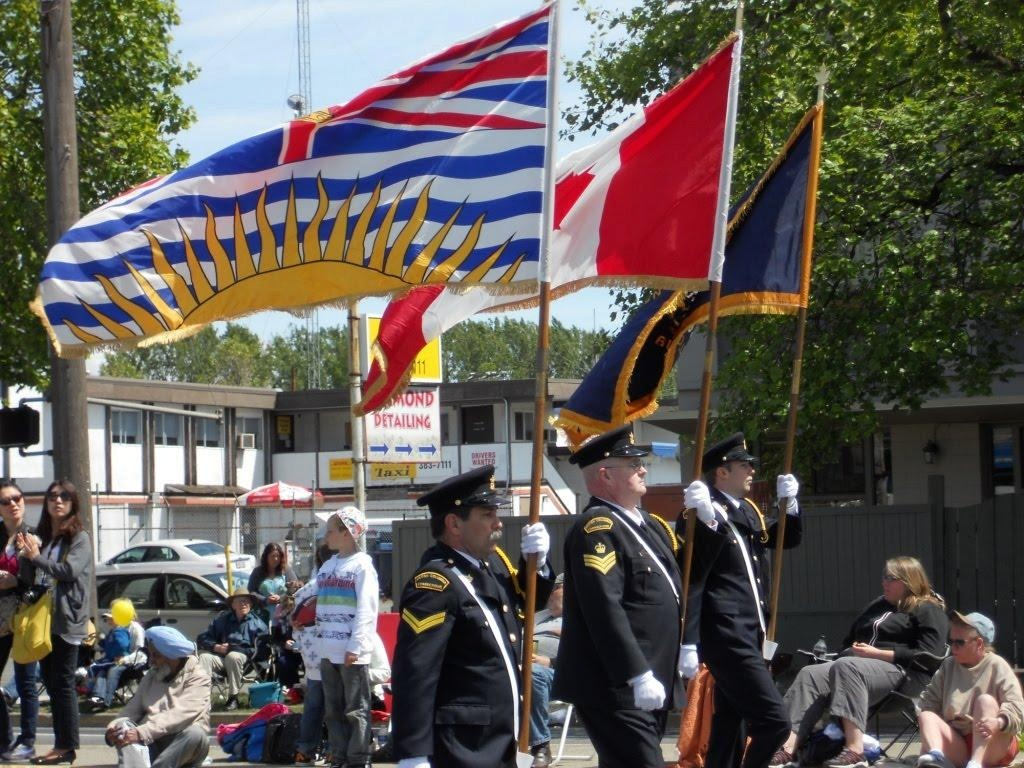
\includegraphics[width=\textwidth]{figures/wider_1}
\end{subfigure}
\begin{subfigure}[b]{0.3\textwidth}
    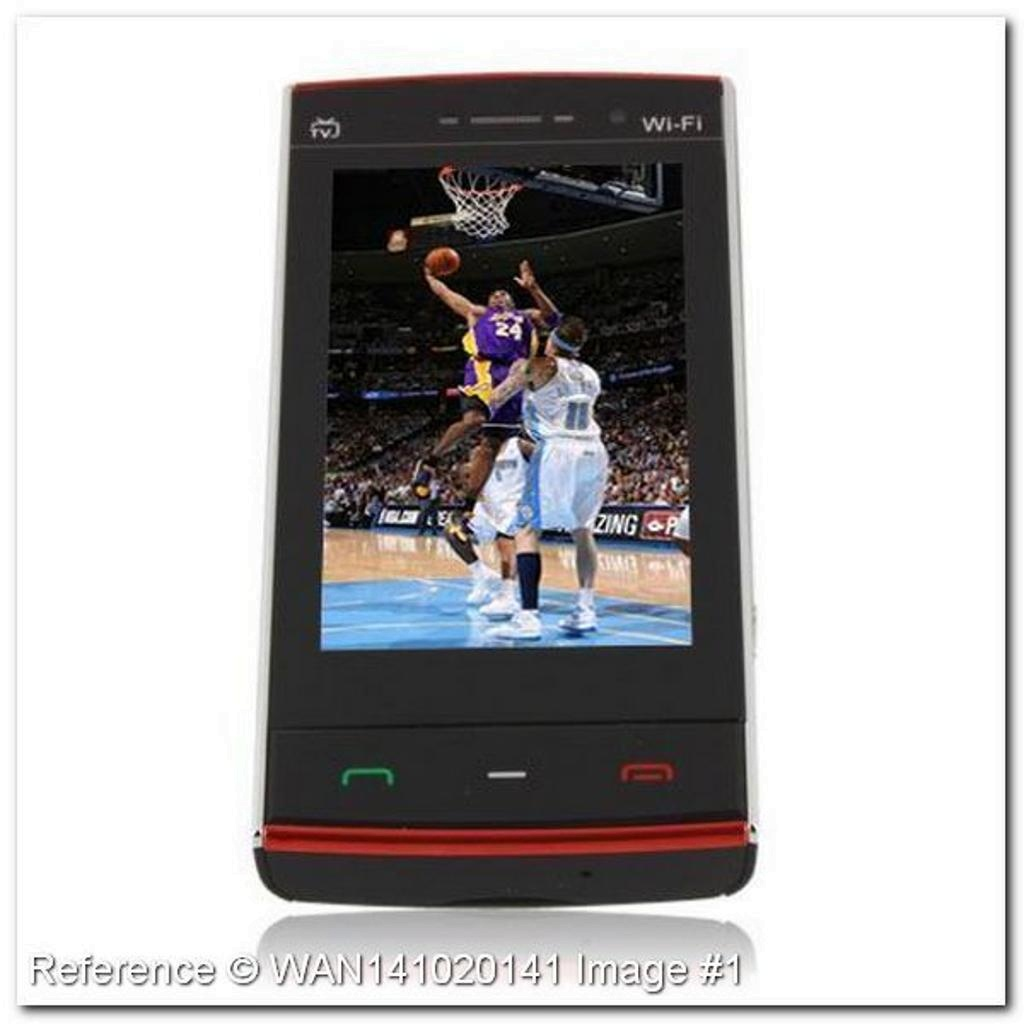
\includegraphics[width=\textwidth]{figures/wider_2}
\end{subfigure}
\begin{subfigure}[b]{0.3\textwidth}
    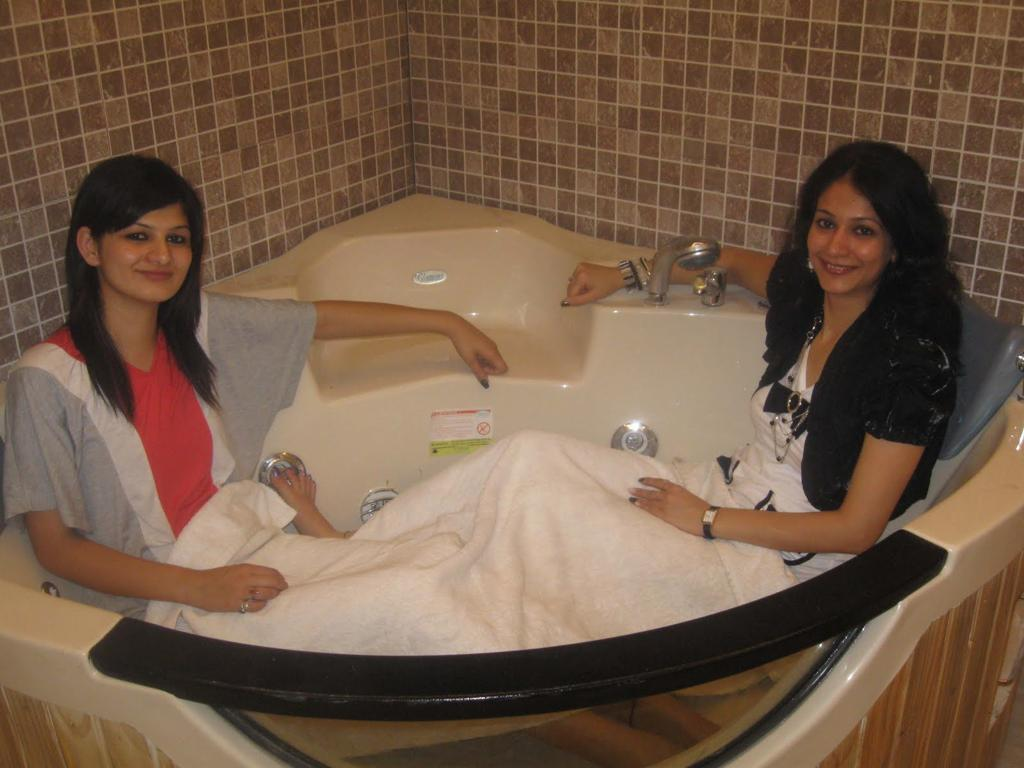
\includegraphics[width=\textwidth]{figures/wider_3}
\end{subfigure}
\begin{subfigure}[b]{0.3\textwidth}
    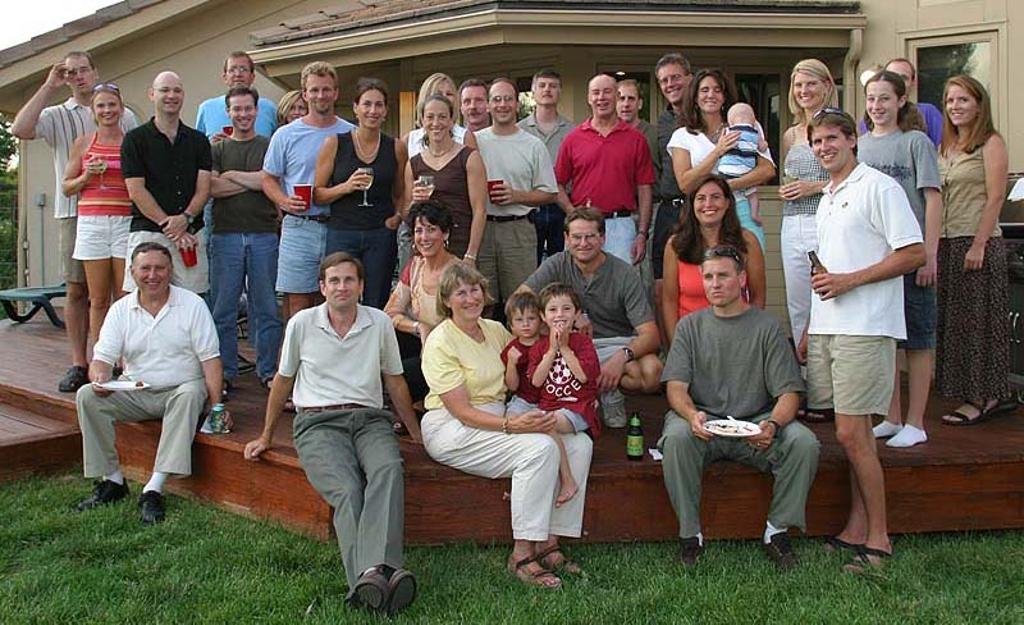
\includegraphics[width=\textwidth]{figures/wider_4}
\end{subfigure}
\begin{subfigure}[b]{0.3\textwidth}
    
\includegraphics[width=\textwidth]{figures/same_original}
\end{subfigure}
\caption[Wider Face 資料集中的圖片範例]{Wider Face 資料集收集了各種不同情境下的人臉}
\label{fig:wider_face}
\end{figure}

訓練時我們使用了 Wider Face~\cite{yang2016wider} 作為主要的資料集。它是一個人臉資料集,其收集了各種不同情境下的人臉 (如圖~\ref{fig:wider_face}),共計 32,203 張圖片、393,703 張人臉,在人臉偵測這個議題上是很經典的資料集。在我們的實驗中,我們將資料集中的圖片分別做了曝光不足和曝光過度的模擬。其中曝光不足的模擬將圖片亮度隨機調為 3\%、5\%、7\%,並將每張圖隨機分配 1 \textasciitilde 10 的數字$n$,以$\sigma = n$的設定對每張圖做高斯雜訊;曝光過度的模擬則將圖片亮度隨機調為 100\%、250\%、400\%。

\begin{figure}[t]
\centering
\begin{subfigure}[b]{0.22\textwidth}
    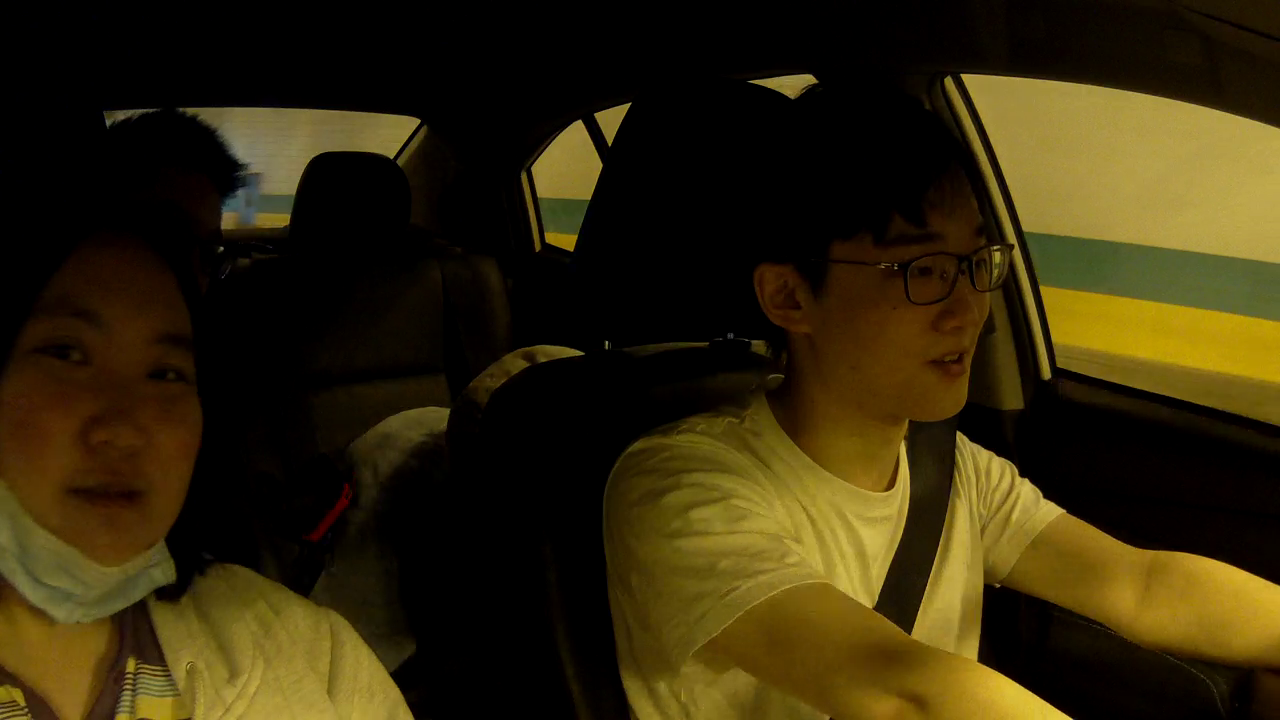
\includegraphics[width=\textwidth]{figures/test_1_1}
\end{subfigure}
\begin{subfigure}[b]{0.22\textwidth}
    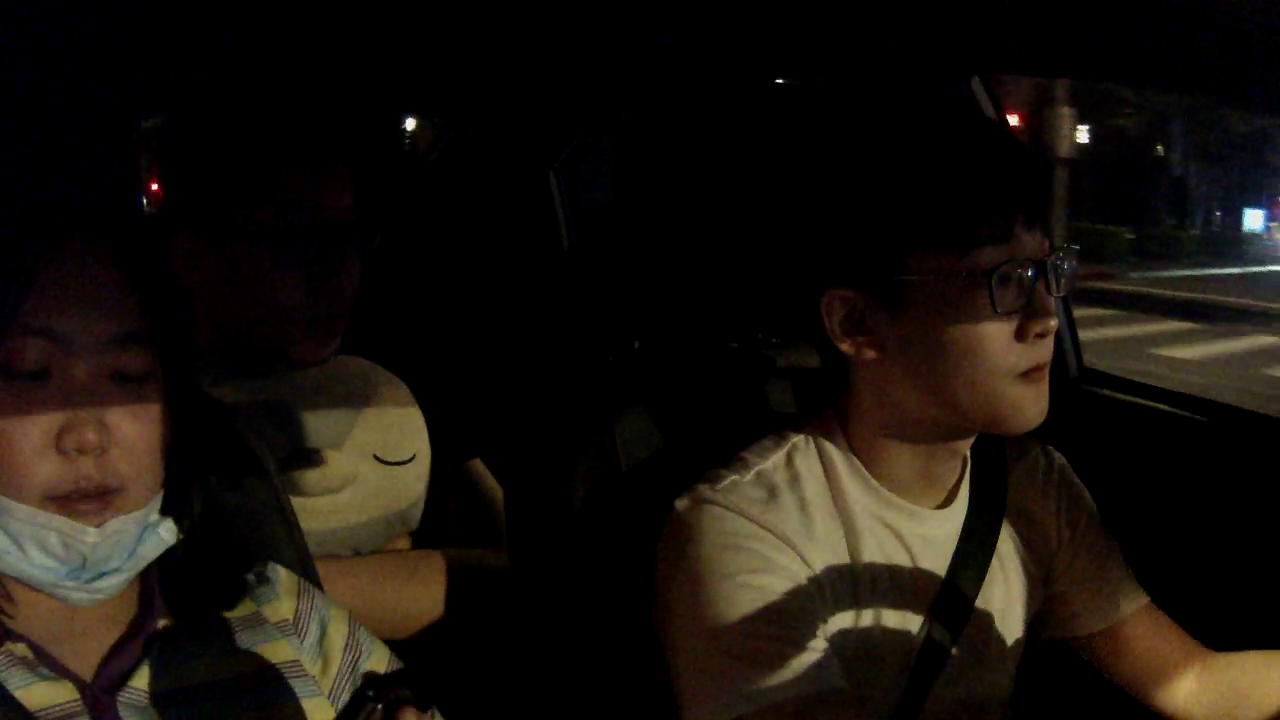
\includegraphics[width=\textwidth]{figures/test_2_1}
\end{subfigure}
\begin{subfigure}[b]{0.22\textwidth}
    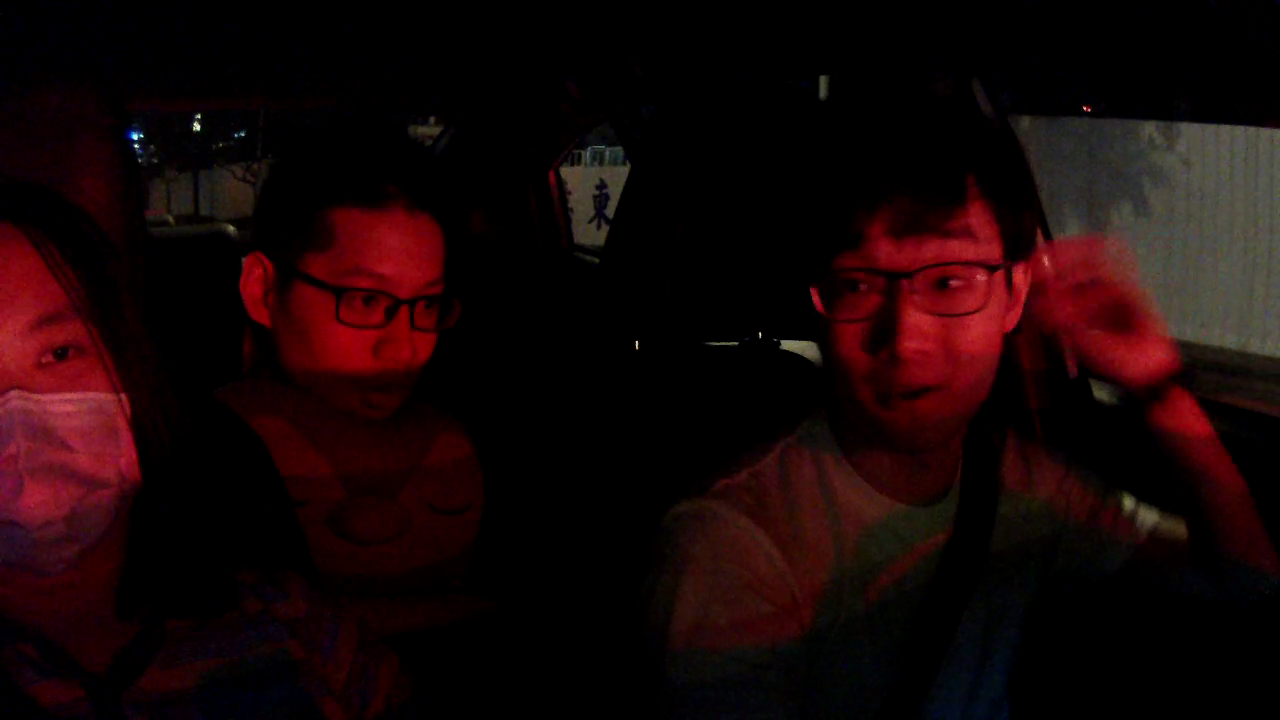
\includegraphics[width=\textwidth]{figures/test_3_1}
\end{subfigure}
\begin{subfigure}[b]{0.22\textwidth}
    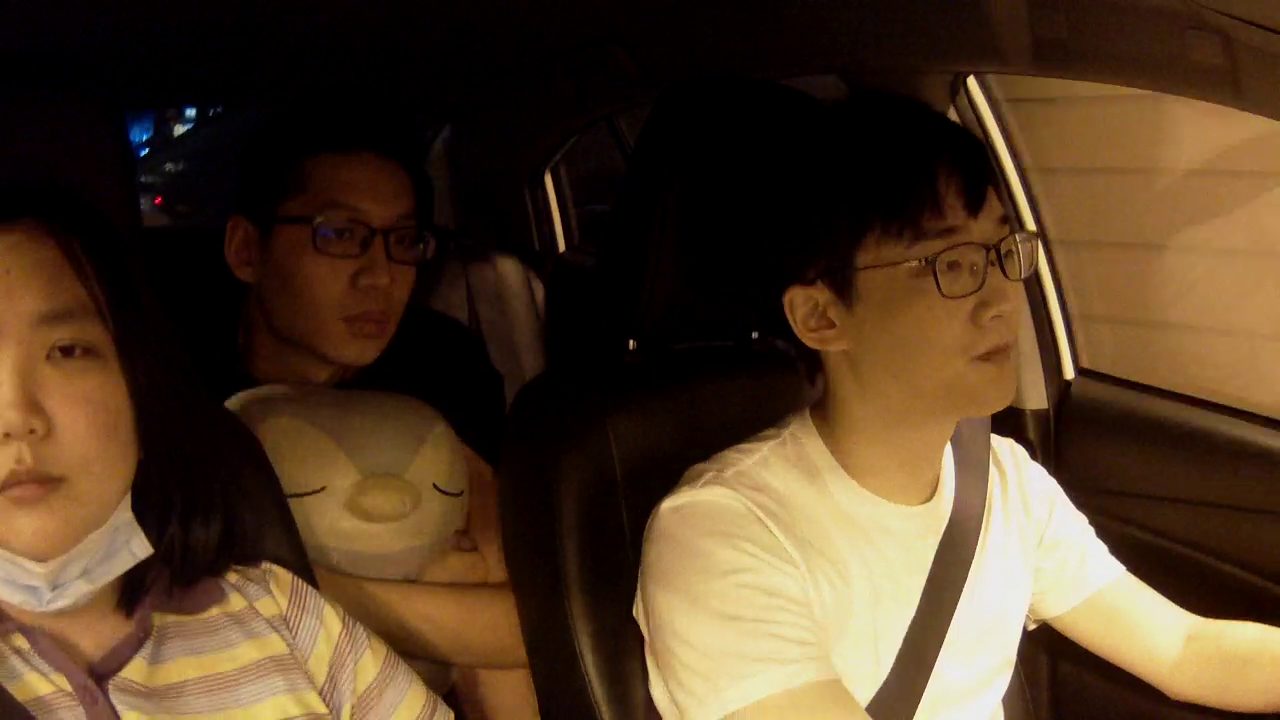
\includegraphics[width=\textwidth]{figures/test_4_1}
\end{subfigure}
\begin{subfigure}[b]{0.22\textwidth}
    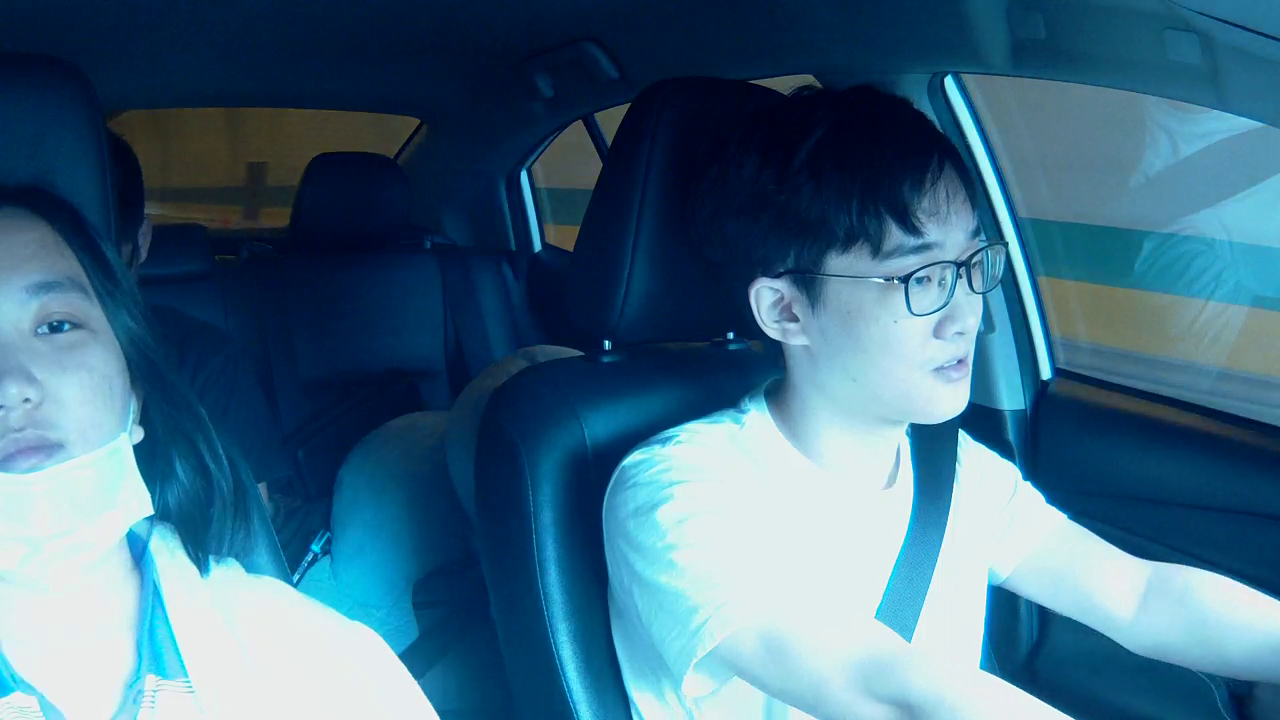
\includegraphics[width=\textwidth]{figures/test_1_2}
    \caption {白天進出隧道}
\end{subfigure}
\begin{subfigure}[b]{0.22\textwidth}
    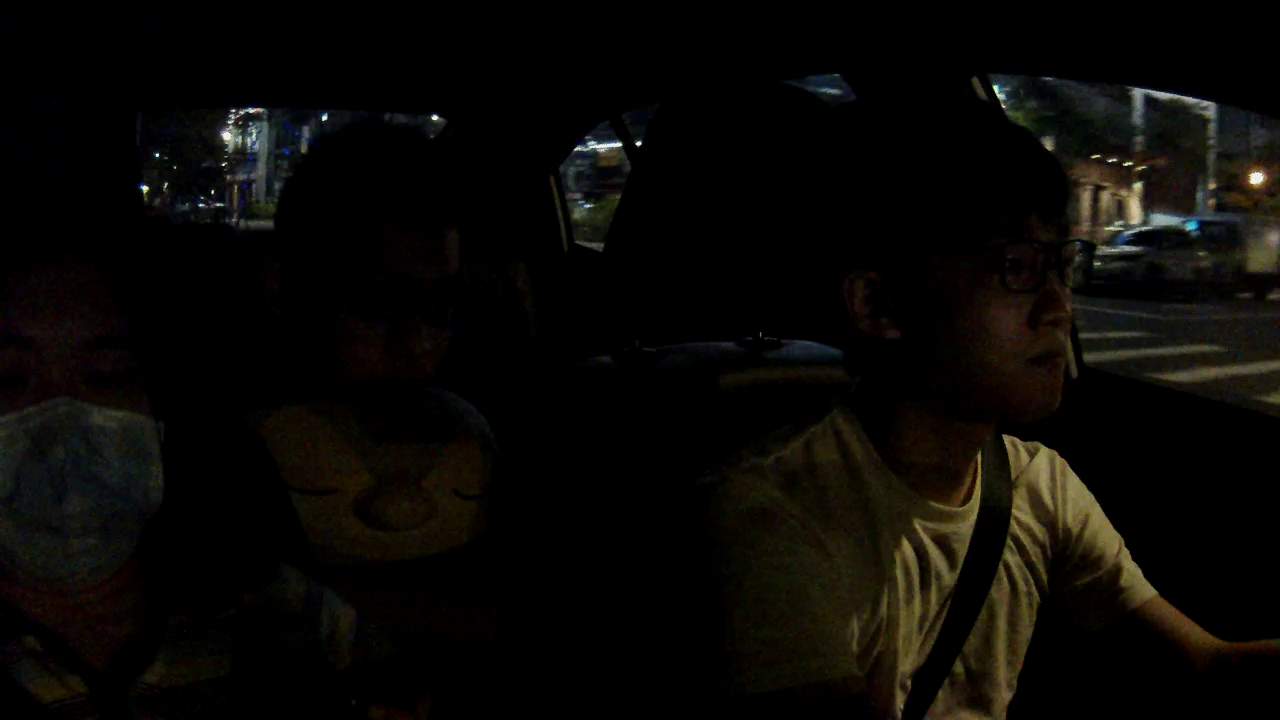
\includegraphics[width=\textwidth]{figures/test_2_2}
    \caption {夜間極暗}
\end{subfigure}
\begin{subfigure}[b]{0.22\textwidth}
    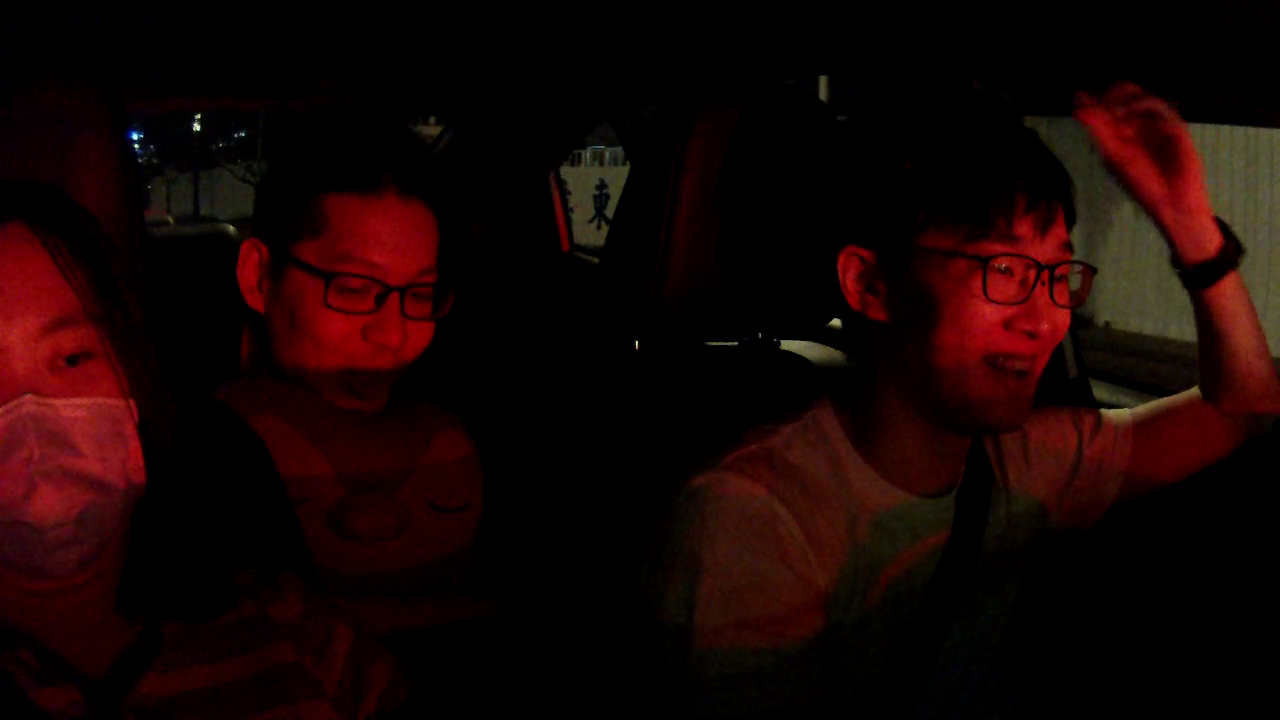
\includegraphics[width=\textwidth]{figures/test_3_2}
    \caption {夜間等紅燈}
\end{subfigure}
\begin{subfigure}[b]{0.22\textwidth}
    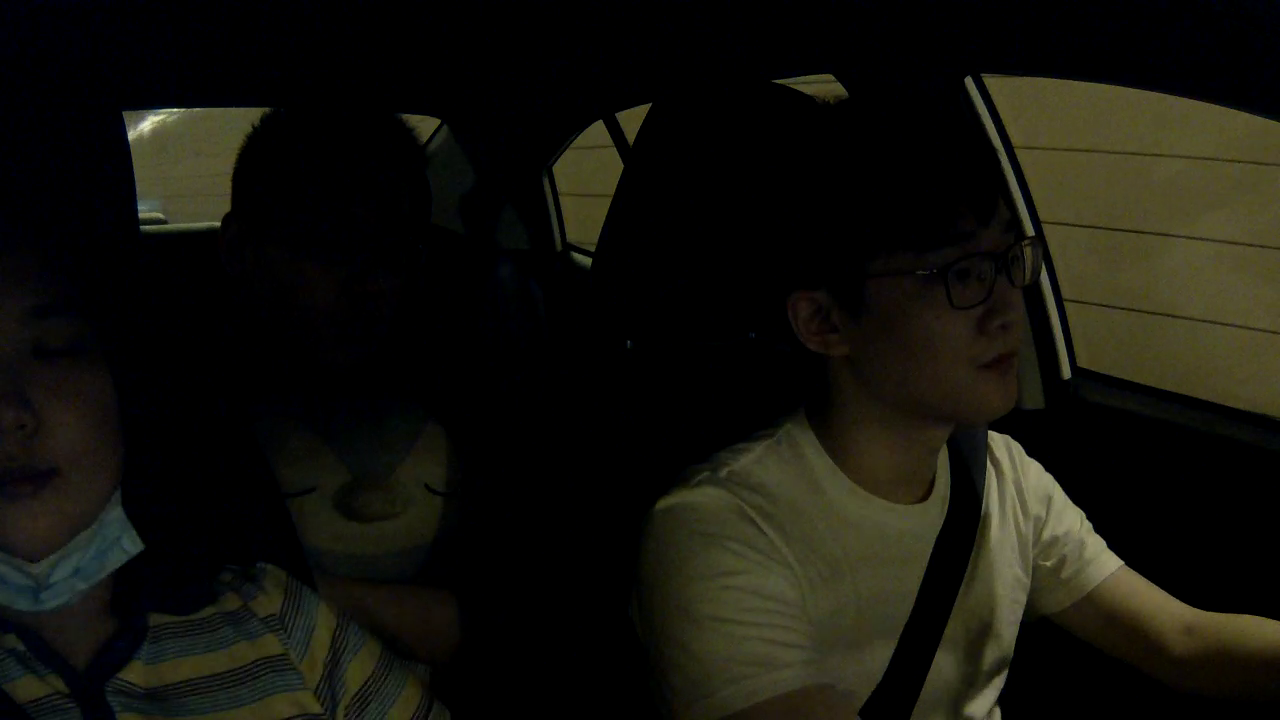
\includegraphics[width=\textwidth]{figures/test_4_2}
    \caption {夜間隧道內}
\end{subfigure}
\caption[測試資料集中的圖片範例]{測試資料集中包含白天進出隧道、夜間極暗、夜間等紅燈和夜間隧道內四個情境}
\label{fig:test_data}
\end{figure}

測試時我們則使用了自己拍攝的車內影像和人工標註的偵測框。我們在進行拍攝時將 Patriot F5 置於前擋風玻璃右上角,影像解析度為$1280 \times 720$,幀率為 30 fps。影像中會出現三個人,包含駕駛、副駕駛、後座的乘客。標註時我們採用和訓練時所使用的 Wider Face 資料集相同的定義,使偵測框緊貼臉部的前額、下巴和臉頰。
此資料集有以下四個情境:白天進出隧道 900 張、夜間極暗 900 張、夜間等紅燈 900 張、夜間隧道內 1000 張 (如圖~\ref{fig:test_data})。白天進出隧道是四個情境中最亮的,用來測試進出隧道時的光線劇烈變化造成的影響;夜間極暗是一個環境光非常微弱的情境,用來測試缺乏環境光造成的影響;夜間等紅燈是一個會受到紅燈直接照射的情境,用來測試資料有色差造成的影響;夜間隧道內是一個隧道光源較微弱的情境,用來測試環境光僅能照亮部分影像造成的影響。在後續的實驗我們也會將這四個情境分開測試。
為求說明方便,後續提到資料集時會使用表~\ref{table:model_names}中對資料集的命名。
\begin{table}[ht]
    \caption{對不同資料集的命名}
    \centering
    \begin{tabular}{l l l}
        \hline
        資料集名稱 & 說明 & 使用時機 \\
        \hline
        $D_{Original}$ & Wider Face 的原始資料集 & - \\
        $D_{Dark}$ & 將 $D_{Original}$ 做曝光不足模擬後的資料集 & - \\
        $D_{Bright}$ & 將 $D_{Original}$ 做曝光過度模擬後的資料集 & - \\
        $D_{Triple}$ & 包含 $D_{Original}$、$D_{Dark}$、$D_{Bright}$ 三個資料集 & 預訓練 \\
        $D_{Train}$	& 包含 $D_{Dark}$ 和 $D_{Bright}$ 兩個資料集 & 主要訓練 \\
        $D_{Test}$ & 我們拍攝的車內影像 & 測試 \\
        \hline
    \end{tabular}
    \label{table:model_names}
\end{table}

\section{實驗設定}

訓練的流程包含預訓練和主要訓練。

在預訓練中,我們使用 $D_{Triple}$ 作為輸入資料集。首先我們將每張圖片調整為 $1024 \times 1024$ 的大小以配合後續訓練要求,然後將圖片切為 256 張 $64 \times 64$ 的小圖片餵進模型以 $\alpha = 0.05$ 進行訓練,經過 30 萬個時期 (Epoch) 後得到正規器在主要訓練中的初始權重。
接著我們進行主要訓練,在這個階段我們使用$D_{Train}$作為輸入資料集,把預訓練中得到的正規器和人臉偵測器接在一起做 150 個時期的端對端訓練。
測試時我們使用 $D_{Test}$ 作為輸入資料集,對其四個情境分別進行測試和結果評估。

\section{實驗結果}

以下會展示用我們的方法測試的結果和用基線測試的結果在數據和視覺上的比較。基線是用將 FaceBoxes 的架構以和原論文中同樣的資料集 ($D_{Original}$) 訓練得到的模型直接對 $D_{Test}$ 進行測試,並已事先測試過該模型做在論文中提到的測試資料上結果和原論文結果相似。
數據上的結果比較如表~\ref{table:baseline_compare},表中數據是我們使用全類平均正確率 (Mean Average Precision) 對偵測結果計算得出的數字,並已經去除部分和本研究無關的結果影響。
\begin{table}[ht]
    \caption{基線和我們的方法之結果比較}
    \centering
    \begin{tabular}{l c c c c}
        \hline
        模型名稱 & 白天進出隧道 & 夜間極暗 & 夜間等紅燈 & 夜間隧道內 \\
        \hline
        基線 (FaceBoxes) & 63.54\% & 31.70\% & 93.35\% & 47.46\% \\
        我們的方法 & 76.25\% & 78.97\% & 97.51\% & 71.66\% \\
        \hline
    \end{tabular}
    \label{table:baseline_compare}
\end{table}

由數據結果可以發現我們的方法得出的結果在環境光較微弱的夜間極暗、夜間隧道內情境下和基線相比分別有 47.27\% 和 24.20\% 的顯著進步,而在白天進出隧道、夜間等紅燈情境下則分別有 12.71\% 和 4.16\% 較小幅的進步。從視覺上的結果 (如圖~\ref{fig:comp_with_base}) 也可看出我們的方法和基線相比能夠偵測出更多曝光不足的人臉,同時兼顧偵測受到正常光線照射下人臉的準確率。

\begin{figure}[t]
\centering
\begin{subfigure}[b]{0.45\textwidth}
    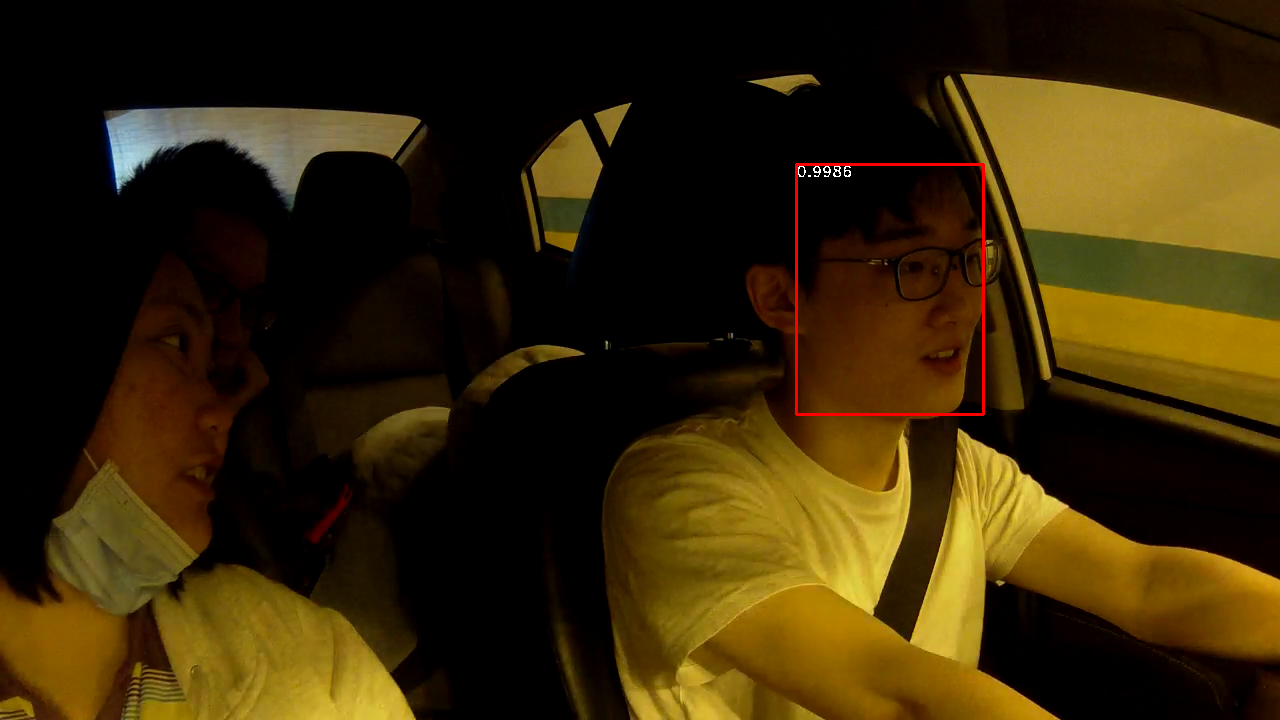
\includegraphics[width=\textwidth]{figures/comp_base1}
\end{subfigure}
\begin{subfigure}[b]{0.45\textwidth}
    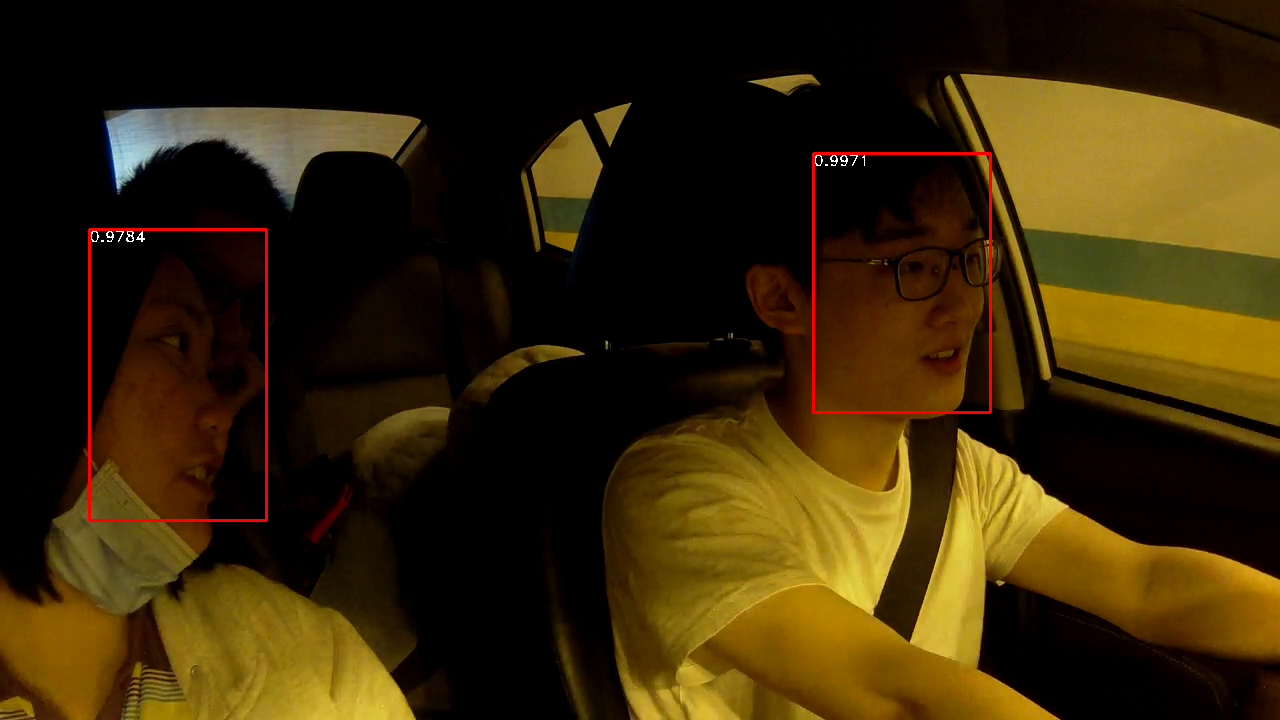
\includegraphics[width=\textwidth]{figures/comp_ours1}
\end{subfigure}
\begin{subfigure}[b]{0.45\textwidth}
    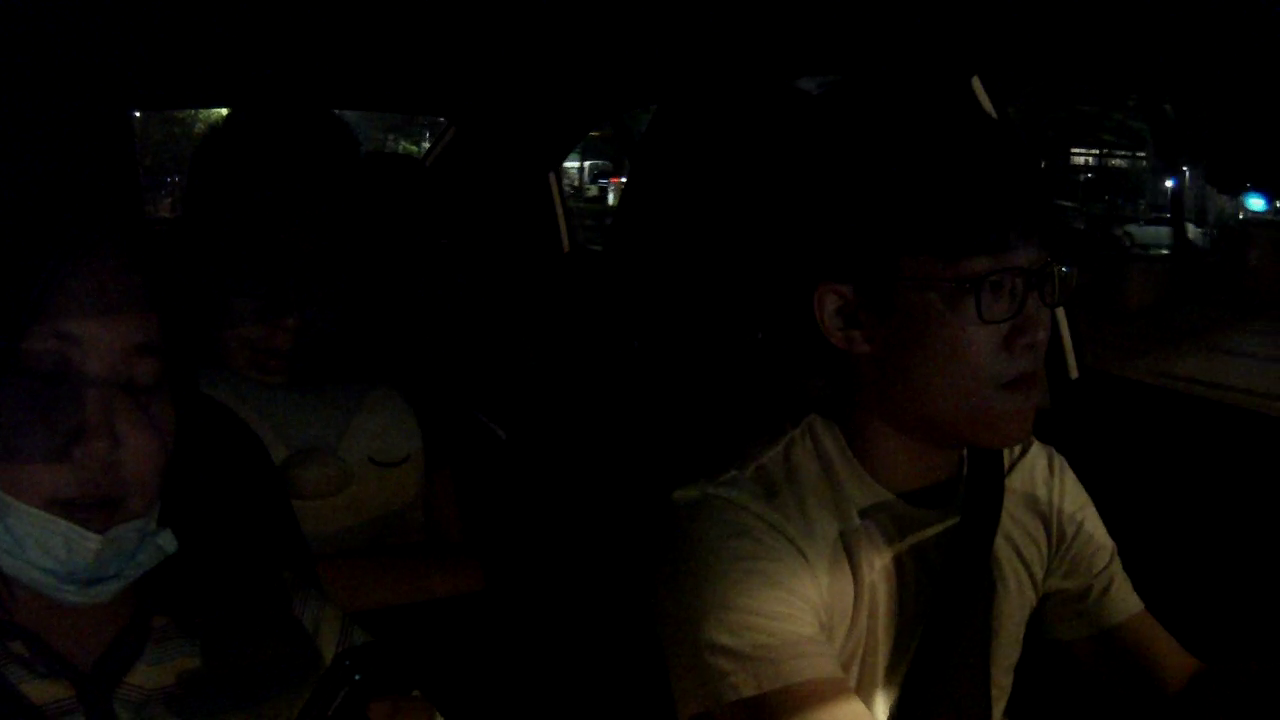
\includegraphics[width=\textwidth]{figures/comp_base2}
\end{subfigure}
\begin{subfigure}[b]{0.45\textwidth}
    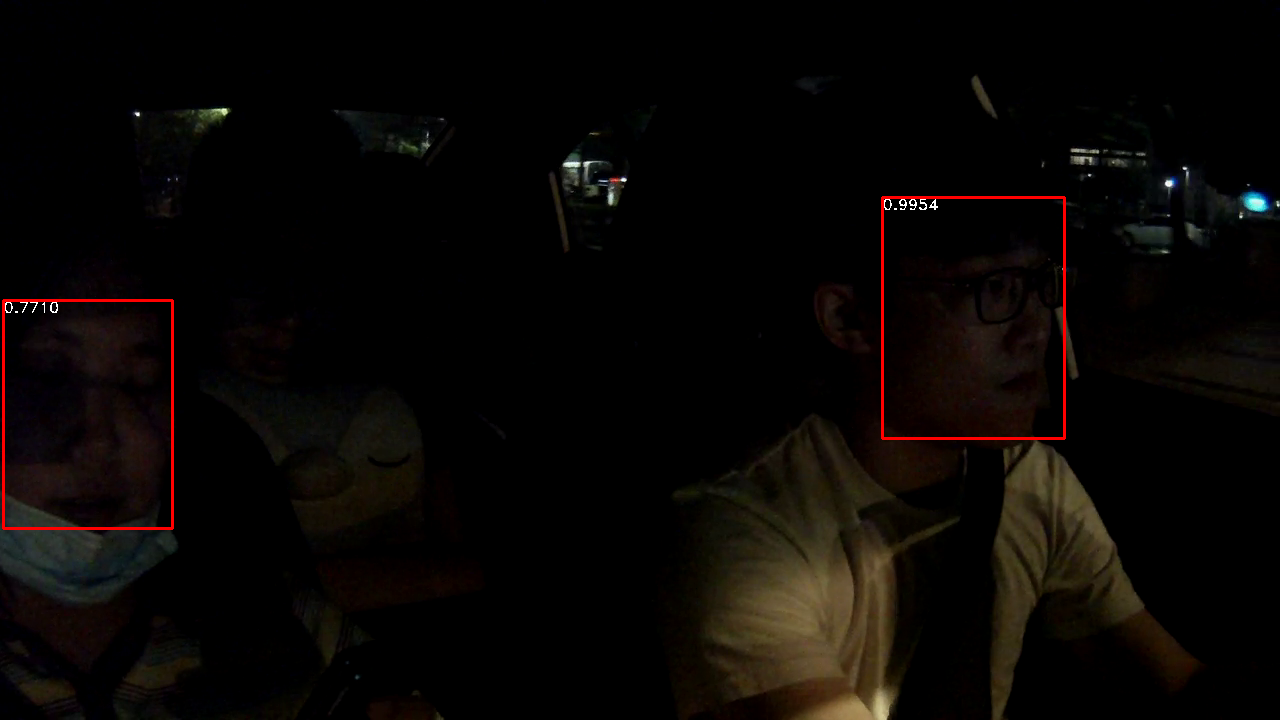
\includegraphics[width=\textwidth]{figures/comp_ours2}
\end{subfigure}
\begin{subfigure}[b]{0.45\textwidth}
    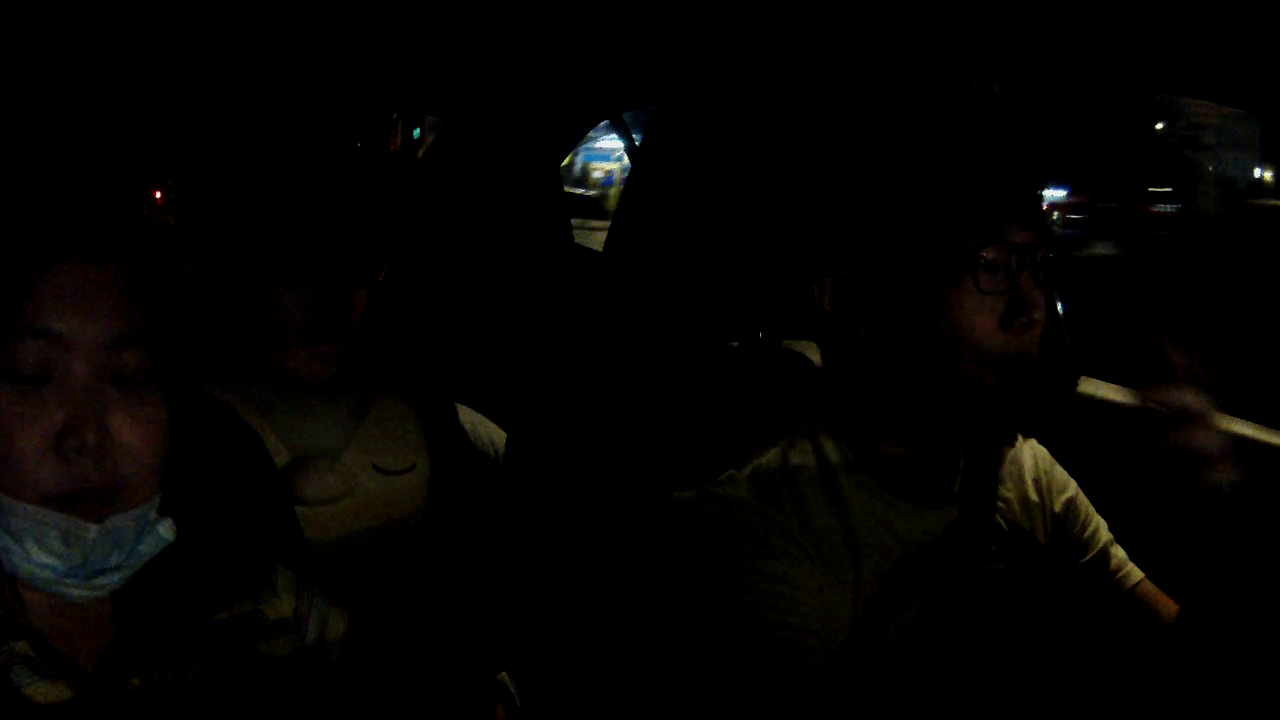
\includegraphics[width=\textwidth]{figures/comp_base3}
\end{subfigure}
\begin{subfigure}[b]{0.45\textwidth}
    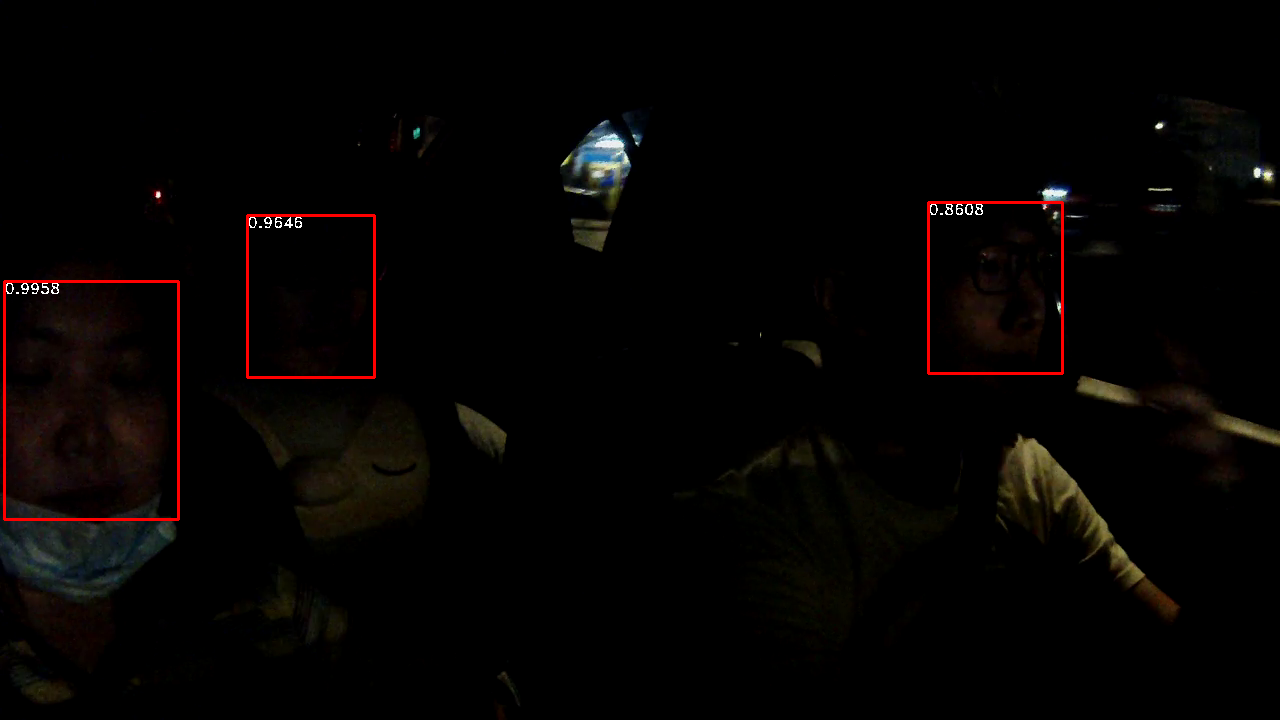
\includegraphics[width=\textwidth]{figures/comp_ours3}
\end{subfigure}
\begin{subfigure}[b]{0.45\textwidth}
    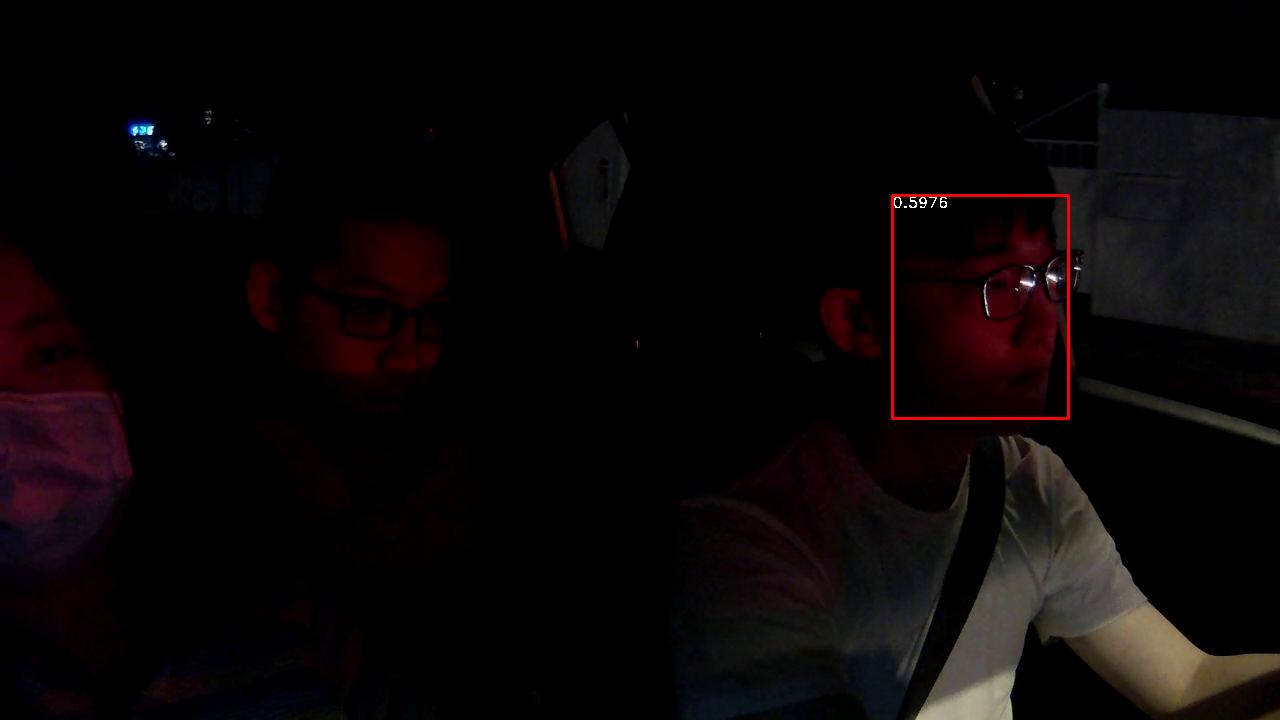
\includegraphics[width=\textwidth]{figures/comp_base4}
\end{subfigure}
\begin{subfigure}[b]{0.45\textwidth}
    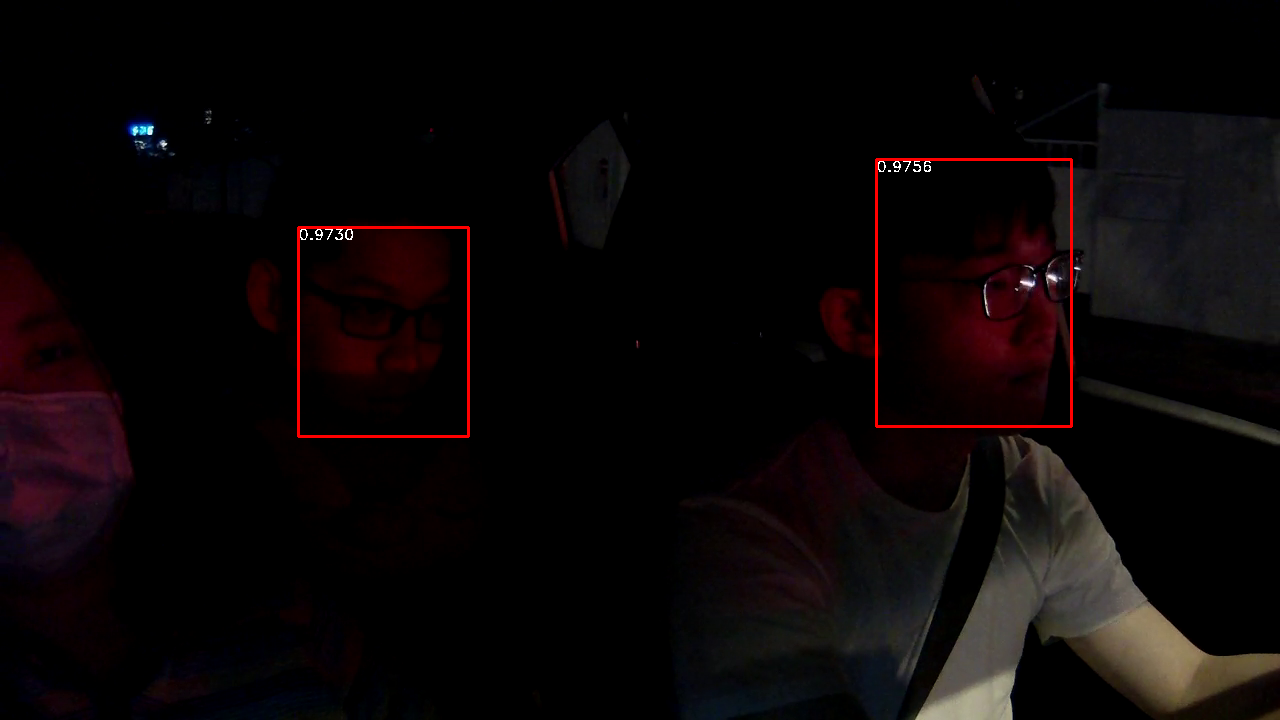
\includegraphics[width=\textwidth]{figures/comp_ours4}
\end{subfigure}
\begin{subfigure}[b]{0.45\textwidth}
    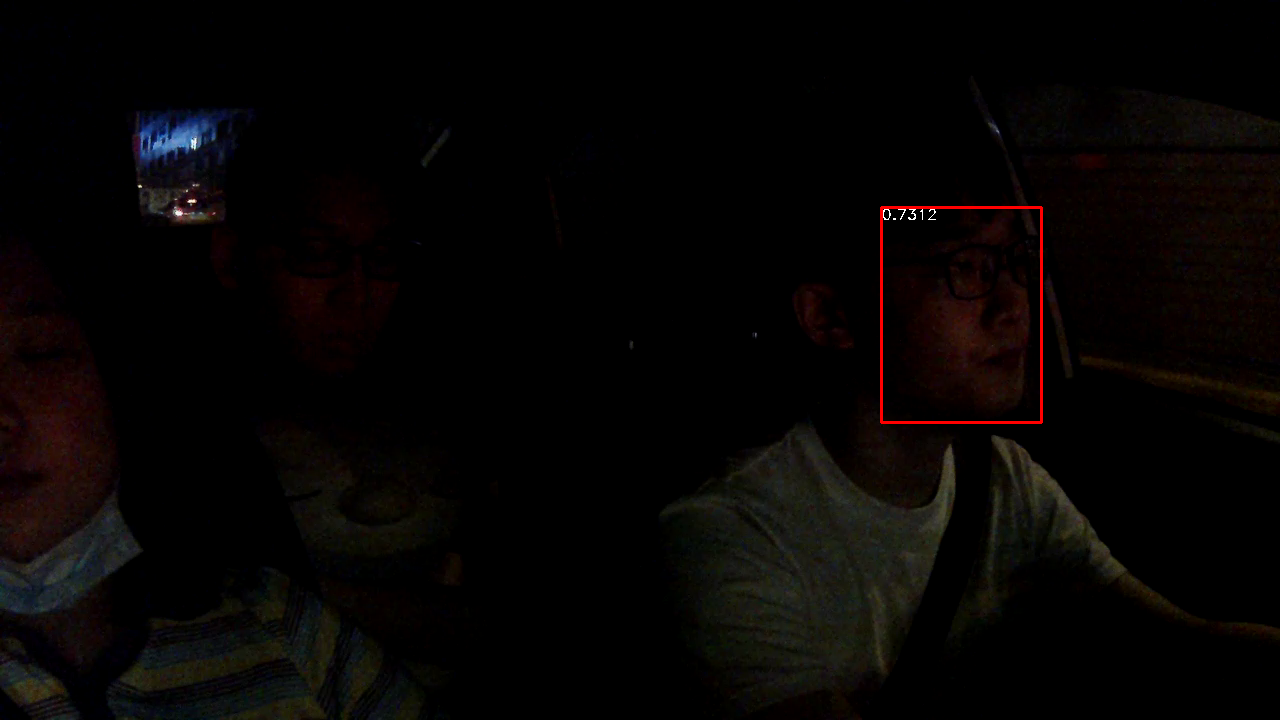
\includegraphics[width=\textwidth]{figures/comp_base5}
\end{subfigure}
\begin{subfigure}[b]{0.45\textwidth}
    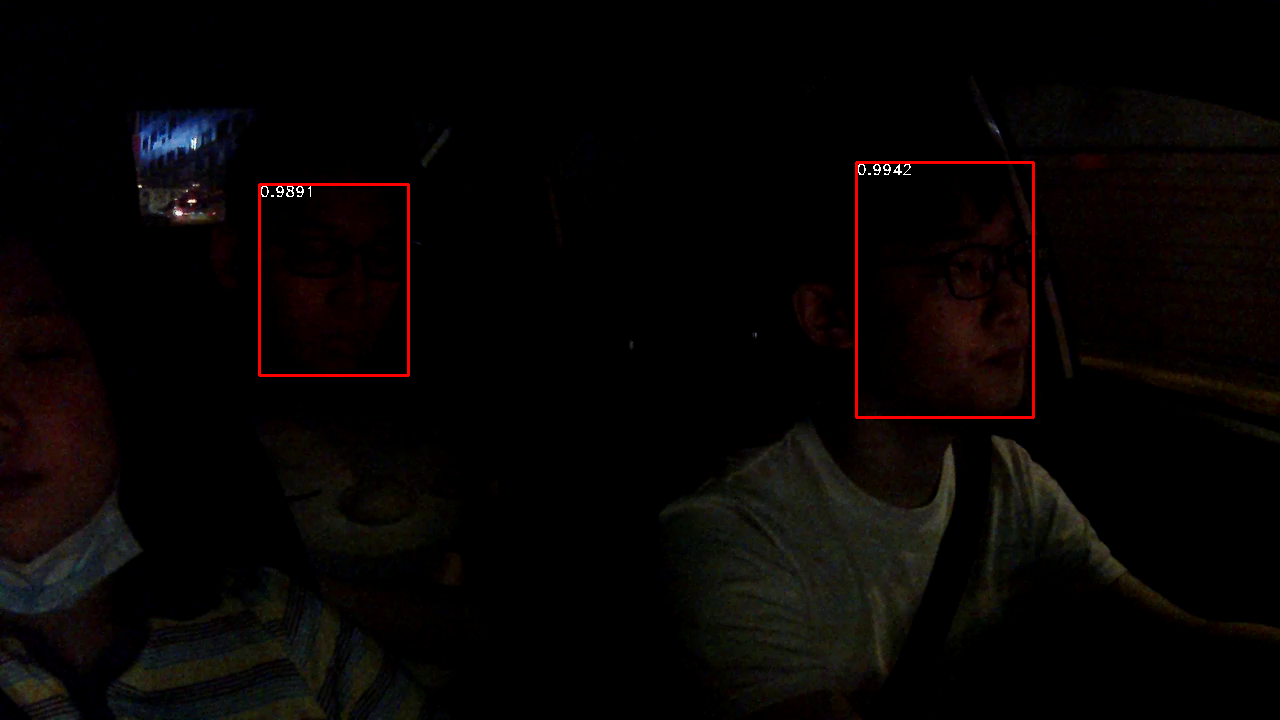
\includegraphics[width=\textwidth]{figures/comp_ours5}
\end{subfigure}
\begin{subfigure}[b]{0.45\textwidth}
    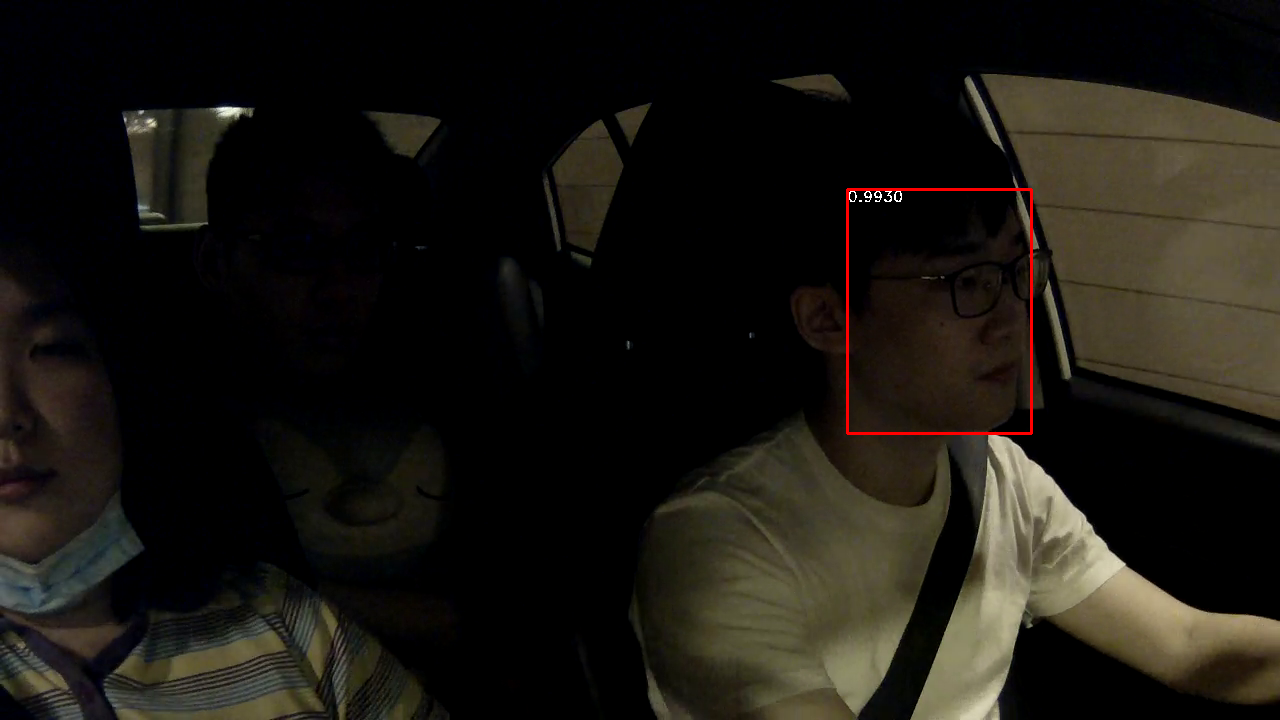
\includegraphics[width=\textwidth]{figures/comp_base6}
    \caption {基線的測試結果}
\end{subfigure}
\begin{subfigure}[b]{0.45\textwidth}
    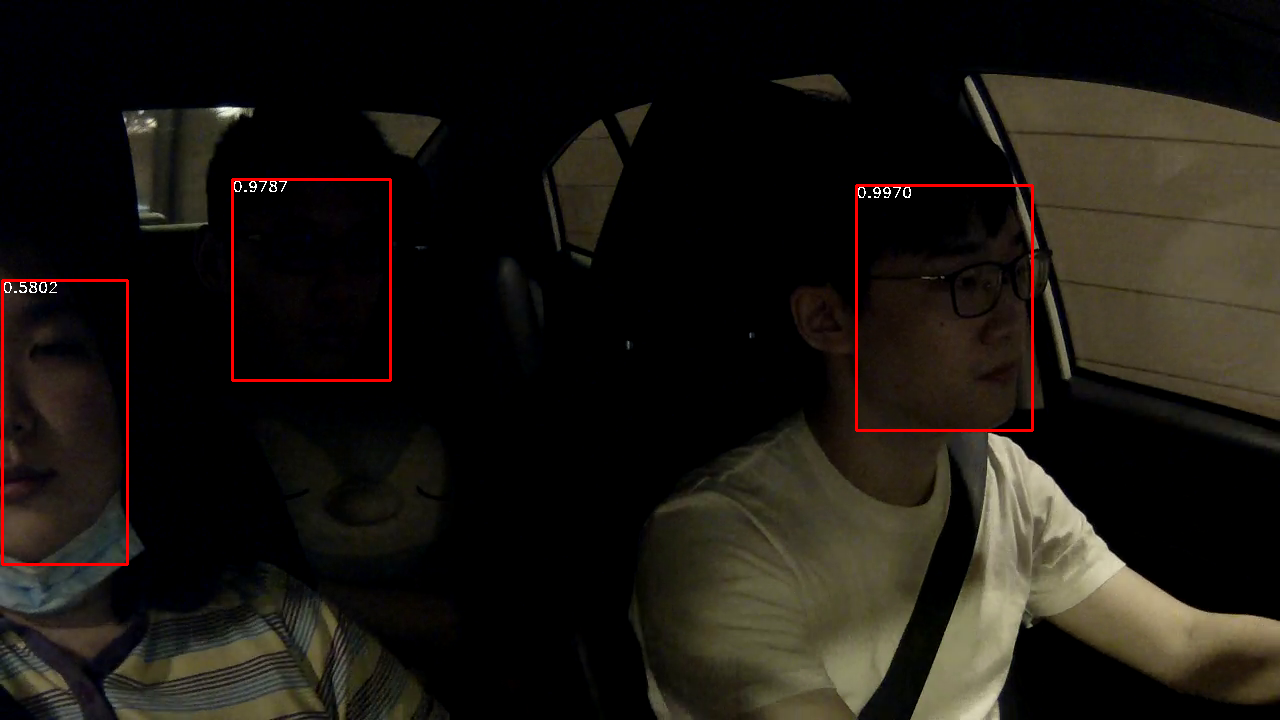
\includegraphics[width=\textwidth]{figures/comp_ours6}
    \caption {我們的方法的測試結果}
\end{subfigure}
\caption[我們的方法與基線之視覺結果比較]{比較我們的方法與基線之視覺結果可發現我們的方法能偵測出更多曝光不足的人臉}
\label{fig:comp_with_base}
\end{figure}

\section{消融實驗}

在這一節,我們會探討我們方法中的每個架構與細節是否真的對車內人偵測有效。我們用 $D_{Test}$ 在不同訓練設定下的模型上作實驗,來確認我們方法中的各個步驟都是有效的。首先我們會先探討在訓練時使用模擬曝光不足 / 曝光過度的資料對實驗結果的影響;接著我們會探討在輸入圖片進行偵測前先進行正規化處理對實驗結果的影響;然後我們會探討在預訓練階段使用三圖一組架構對實驗結果的影響;最後我們會探討在主要訓練階段對正規器繼續進行優化對實驗結果的影響。

\subsection{在訓練時使用模擬曝光不足 / 曝光過度的資料}

在我們的方法中,第一個和基線方法不同的地方在於我們訓練時不是使用 $D_{Original}$ 這個收集了正常光照下圖片的資料集,而是使用了將 $D_{Original}$ 模擬曝光不足情境生成的 $D_{Dark}$ 和模擬曝光過度情境生成的 $D_{Bright}$ 合在一起的 $D_{Train}$作為訓練資料集。因此首先我們要先探討這件事是否有效。

由於我們的方法的架構中有正規器,以 $D_{Original}$ 作為訓練資料集意義不大,同時為了去除其他部分對模型造成的影響,最後我們選擇比較\textbf{基線}和\textbf{對照組 A} 這兩個不同訓練設定下的實驗結果如表~\ref{table:data_compare}。
對照組 A 的模型架構只包含人臉偵測器而沒有對輸入圖片進行正規化處理,以 $D_{Train}$ 作為訓練資料集。
兩者差別在於主要訓練階段所使用的資料集不同。基線設定以 $D_{Original}$ 作為訓練資料集;對照組 A 設定則使用了經過演算法模擬曝光不足 / 曝光過度的圖片,以 $D_{Train}$ 作為訓練資料集。

\begin{table}[ht]
    \caption{在訓練時使用模擬曝光不足 / 曝光過度的資料對測試結果的影響}
    \centering
    \begin{tabular}{l c c c c}
        \hline
        設定名稱 & 白天進出隧道 & 夜間極暗 & 夜間等紅燈 & 夜間隧道內 \\
        \hline
        基線 & 63.54\% & 31.70\% & 93.35\% & 47.46\% \\
        對照組 A & 70.97\% & \textbf{63.16\%} & 90.75\% & 62.73\% \\
        \hline
    \end{tabular}
    \label{table:data_compare}
\end{table}

從數據上的結果我們可以得知,對照組 A 設定和基線設定相比在白天進出隧道情境有 7.43\% 的進步,在夜間隧道內情境有 15.27\% 的進步,而在環境光非常微弱的夜間極暗情境更是有 31.46\% 的進步。
我們認為這代表使用較極端光線照射下的圖片作為輸入資料有助於讓偵測器在訓練階段認識更多在不同光線照射下的人臉,使我們在測試階段能夠偵測出更多原本受到光照影響而不認識的人臉。

\subsection{在偵測前進行正規化處理}

在我們的方法中,我們在偵測對輸入圖片進行了正規化處理。接下來我們會探討這一步對實驗結果的影響。
我們比較\textbf{對照組 A}、\textbf{對照組 B}、\textbf{對照組 C}、\textbf{我們的方法}這四個不同訓練設定下的實驗結果如表~\ref{table:normalize_compare}。

對照組 A 如上一小節所述,是以 $D_{Train}$ 作為訓練資料集,整個模型架構只包含人臉偵測器,沒有對輸入圖片進行正規化處理的設定。
對照組 B 在預訓練階段盡可能還原了我們所使用的正規器模型架構 MSR-net~\cite{shen2017msr} 的訓練設定,以 $D_{Dark}$ 作為預訓練的訓練資料集,以用視網膜增強算法對 $D_{Dark}$ 的圖片進行處理後的結果圖片作為基準真相,對正規器進行預訓練。接著在主要訓練階段,我們以 $D_{Train}$ 作為訓練資料集,對正規器和人臉偵測器進行端對端訓練。
對照組 C 在預訓練階段使用了第~\ref{c:method}章圖~\ref{fig:original_pretrain}所提到的架構,以包含了 $D_{Dark}$ 和 $D_{Bright}$ 的 $D_{Train}$ 作為預訓練資料集、$D_{Original}$ 作為基準真相,讓正規器進行監督式學習。接著在主要訓練階段,我們以 $D_{Train}$ 作為訓練資料集,對正規器和人臉偵測器進行端對端訓練。
我們的方法在預訓練階段以包含了$D_{Dark}$、$D_{Bright}$、$D_{Original}$ 的 $D_{Triple}$ 作為預訓練資料集,採用三圖一組的架構 (如圖~\ref{fig:triple_setting}),以迂迴的方式對正規器進行預訓練。接著在主要訓練階段,我們以 $D_{Train}$ 作為訓練資料集,對正規器和人臉偵測器進行端對端訓練。

除了對照組 A 之外的其他設定分別採用了不同架構或設定對正規器進行預訓練,但三者之間共通的是都有對輸入圖片進行正規化處理,僅對照組 A 沒有。

\begin{table}[ht]
    \caption{針對在偵測前進行正規化處理與否之比較}
    \centering
    \begin{tabular}{l c c c c}
        \hline
        設定名稱 & 白天進出隧道 & 夜間極暗 & 夜間等紅燈 & 夜間隧道內 \\
        \hline
        對照組 A & \emph{70.97\%} & \emph{63.16\%} & \emph{90.75\%} & \emph{62.73\%} \\
        \hline
        對照組 B & 74.66\% & 81.21\% &95.42\% & 69.54\% \\
        對照組 C & 73.56\% & 76.02\% & 96.59\% & 68.73\% \\
        我們的方法 & 76.25\% & 78.97\% & 97.51\% & 71.66\% \\
        \hline
    \end{tabular}
    \label{table:normalize_compare}
\end{table}

從數據上的結果我們可以看到,對輸入圖片進行過正規化的設定無一例外都獲得了比對照組 A 更好的結果。
這能夠證明對輸入資料進行正規化處理對人臉偵測有幫助,並且在環境光較微弱的情境下這個影響更加明顯,如在夜間極暗情境下,對照組 B、對照組 C、我們的方法和對照組 A 相比,分別有 18.05\%、12.86\%、15.81\% 的進步。
我們認為這代表正規化處理成功將不同光照下的圖片內容進行調整使其有相似的長相,讓後續的偵測過程更加順利。
特別要注意的是,雖然我們的方法和對照組 B 相比在夜間極暗情境下有 2.24\% 的些微退步,但這個情境的環境光極度微弱,在部分圖片中兩者都只有抓出人臉的一部分,而有些偵測框碰巧跨過了 $IOU >=50\%$ 的門檻。實際上這兩個設定在這個情境下視覺上相差並不大。

\subsection{使用三圖一組架構進行預訓練}

接著我們希望能證明,我們在預訓練階段所使用的三圖一組架構對人臉偵測是有幫助的。為此我們比較\textbf{對照組 C} 和\textbf{我們的方法}這兩個不同訓練設定下的實驗結果如表~\ref{table:triple_compare}。兩個設定的詳細訓練設定在上一小節已經詳述,這裡不再贅述。
兩個設定都會對輸入圖片進行正規化處理,也都有對正規器進行預訓練,預訓練階段所用到的資料集也相同。它們唯一的差別在於預訓練階段所使用的訓練架構。
對照組 C 直接讓正規器進行監督式學習,而我們的方法則使用三圖一組架構迂迴地訓練正規器。

\begin{table}[ht]
    \caption{針對使用三圖一組架構進行預訓練的效果之比較}
    \centering
    \begin{tabular}{l c c c c}
        \hline
        設定名稱 & 白天進出隧道 & 夜間極暗 & 夜間等紅燈 & 夜間隧道內 \\
        \hline
        對照組 C & 73.56\% & 76.02\% & 96.59\% & 68.73\% \\
        我們的方法 & 76.25\% & 78.97\% & 97.51\% & 71.66\% \\
        \hline
    \end{tabular}
    \label{table:triple_compare}
\end{table}

數據上的結果顯示,即使兩個設定都有對正規器進行預訓練,在後續的主要訓練階段也都有進行端對端訓練優化,且在預訓練階段用到的資料集、主要訓練階段使用的資料集和訓練設定等都一致,我們的方法卻有比較好的結果,在四個測試情境下分別進步了 2.69\%、2.95\%、0.92\%、2.87\%。
在第~\ref{c:method}章我們也提過,由於主要訓練階段的需要,我們在預訓練階段所使用的模型架構有較少的參數也較弱,因此對照組 C 的架構無法順利訓練出我們想要的結果。但在我們更動架構後,我們成功獲得了較佳的偵測結果。我們認為這代表預訓練時三圖一組的架構能夠有效降低模型學習如何對圖片進行正規化處理的難度,使訓練結果更容易收斂。

\subsection{在預訓練後對正規器進行端對端訓練優化}

最後我們探討在主要訓練階段對正規器進行端對端訓練優化的必要性。

我們分別比較兩對設定:\textbf{對照組 D} 和\textbf{對照組 B}、\textbf{對照組 E} 和\textbf{我們的方法} 以及\textbf{對照組 A} 這幾個不同訓練設定下的實驗結果如表~\ref{table:optimize_compare}。
對照組 A、對照組 B、我們的方法的詳細設定在前面都已經詳述,這裡不再贅述。
對照組 D 在預訓練階段和對照組 B 完全一致,盡可能還原了 MSR-net 的訓練設定進行預訓練。但在主要訓練階段,我們凍結了正規器的權重,只更新人臉偵測器部分的權重。
對照組 E 在預訓練階段和我們的方法完全一致,使用了三圖一組架構對正規器進行預訓練。但在主要訓練階段,我們凍結了正規器的權重,只更新人臉偵測器部分的權重。
兩對設定有一個共通點,就是都有一個設定 (對照組 D 和對照組 E) 在主要訓練時凍結了正規器的權重,只訓練人臉偵測器本身。對照組 A 在這個比較中則作為沒有用到正規器的對照組。

\begin{table}[ht]
    \caption{不同設定間之結果比較}
    \centering
    \begin{tabular}{l c c c c}
        \hline
        設定名稱 & 白天進出隧道 & 夜間極暗 & 夜間等紅燈 & 夜間隧道內 \\
        \hline
        對照組 A (無正規器) & 70.97\% & 63.16\% & 90.75\% & 62.73\% \\
        \hline
        對照組 D (未優化) & 73.15\% & \emph{60.13\%} & \emph{88.67\%} & 63.88\% \\
        對照組 B (有優化) & 74.66\% & 81.21\% & 95.42\% & 69.54\% \\
        \hline
        對照組 E (未優化) & \emph{22.61\%} & \emph{41.13\%} & \emph{83.31\%} & \emph{30.35\%} \\
        我們的方法 (有優化) & 76.25\% & 78.97\% & 97.51\% & 71.66\% \\
        \hline
    \end{tabular}
    \label{table:optimize_compare}
\end{table}

數據上的結果顯示,光是進行正規器的預訓練是不夠的。如果不進行後續的優化,結果可能反而會比不進行正規化處理還要差。
我們推測這是由於正規器對圖片進行的調整雖然拉近了不同光照下圖片間的距離,卻增加了一些本不應存在的雜訊或使圖片產生了不該有的色偏,使得偵測器無法順利偵測出人臉。但預訓練依然給了正規器一個好的初始權重,讓模型知道這樣調整圖片可以拉近彼此間的距離。
而端對端訓練的意義便在於對正規器做的事情進行調整與優化,使它在拉近圖片間距離的同時顧及偵測器對人臉偵測的需求。

在經過以上的測試後,我們確認了我們的方法中的各個步驟都是有效的。
\chapter{總結與未來目標}
\label{c:conclusion}

在本研究中,我們提出了基於三元組概念的預訓練架構來訓練出能將不同光線照射下的圖片正規化成相似結果的正規器,並將正規器和人臉偵測器接在一起做端對端訓練優化來提升人臉偵測的準確率。實驗表明我們的方法對正規器的訓練有幫助,也提升了整體人臉偵測的準確率。

未來我們能夠改進的地方包含了以下幾點:我們能夠修改三元組訓練架構中的損失函數,使其能將圖片的正規化處理做得更好;我們還能修改模擬曝光不足、曝光過度圖片的演算法,使其能夠更貼近真實圖片的樣貌以利訓練進行。


\appendix

\backmatter

\addcontentsline{toc}{chapter}{\bibname}
\bibliographystyle{abbrv}

% Your bibliography goes here
\bibliography{thesis}

\end{document}
